%% V1.0
%% by Gabriel Garcia, gabrcg@gmail.com
%% This is a template for Udacity projects using IEEEtran.cls

%% Be Udacious!

\documentclass[10pt,journal,compsoc]{IEEEtran}

%------------------------------------------------------

\usepackage[pdftex]{graphicx}  
\usepackage{cite}
\hyphenation{op-tical net-works semi-conduc-tor}
\usepackage[a4paper, total={6in, 9in}]{geometry}
\usepackage{amsmath}
\usepackage{booktabs}
\usepackage{caption}
\usepackage{enumitem}
\usepackage{graphicx}
\usepackage{float}
\usepackage{inconsolata}
\usepackage{listings}
\usepackage{pstricks-add}
\usepackage{siunitx}
\usepackage[most]{tcolorbox}
\usepackage{tikz}
\usepackage{epstopdf} %converting to PDF
\usepackage[hidelinks]{hyperref}
\usepackage{makecell}
\usepackage{siunitx}
\usepackage{wrapfig}

\usetikzlibrary{shapes.geometric}

%-------------------------------------------------------
\graphicspath{{./fig/}}

%-------------------------------------------------------
\setlength{\parindent}{0in}

\lstdefinestyle{Python}{
	language        = Python,
	basicstyle      = \ttfamily,
	keywordstyle    = \color{blue},
	keywordstyle    = [2] \color{teal}, % just to check that it works
	stringstyle     = \color{green},
	commentstyle    = \color{red}\ttfamily
}

%-------------------------------------------------------
\newtcblisting[auto counter]{sexylisting}[2][]{sharp corners, 
	fonttitle=\bfseries, colframe=gray, listing only, 
	listing options={basicstyle=\ttfamily,language=Python}, 
	title=Listing \thetcbcounter: #2, #1}

%-------------------------------------------------------


\begin{document}
	
	\title{Solar Panel Soiling State Classification}
	
	\author{Shane Reynolds}
	
	\markboth{Inference project}%
	{}
	\IEEEtitleabstractindextext{%
		
		\begin{abstract}
			Solar energy investment is seeing an increased focus as Australia tries to reduce its carbon footprint. One of the main challenges with generation from large solar arrays is keeping the solar panels free from soiling, to limit power loss. This paper aims to develop a solar panel soiling state classification model based on Convolutional Neural Network architectures. Training data is collected using Google image search. Implemented models are based on Googlenet architectures which demostrate mixed results, suggesting the need for more data to increase predictive capabilities.
		\end{abstract}
		
		% Note that keywords are not normally used for peerreview papers.
		\begin{IEEEkeywords}
			Convolutional Neural Network, Deep Learning, Solar Array.
		\end{IEEEkeywords}}
		
		
		\maketitle
		\IEEEdisplaynontitleabstractindextext
		\IEEEpeerreviewmaketitle
		\section{Introduction}
		\label{sec:introduction}
		
		\IEEEPARstart{A}{ustralia} has the highest average solar radiation per square metre of any continent in the world. There is approximately 58 million petajoules of incident solar radiation on Austrlian soil annually - enough to meet Australia's energy demands by a multiple of 10000 \cite{Australia:2014}. Historically, Australia has used coal as its the main source of generation. Solar resources have remained largely unused - this is in line with global trends in energy consumption.
		\begin{figure}[h]
			\centering
			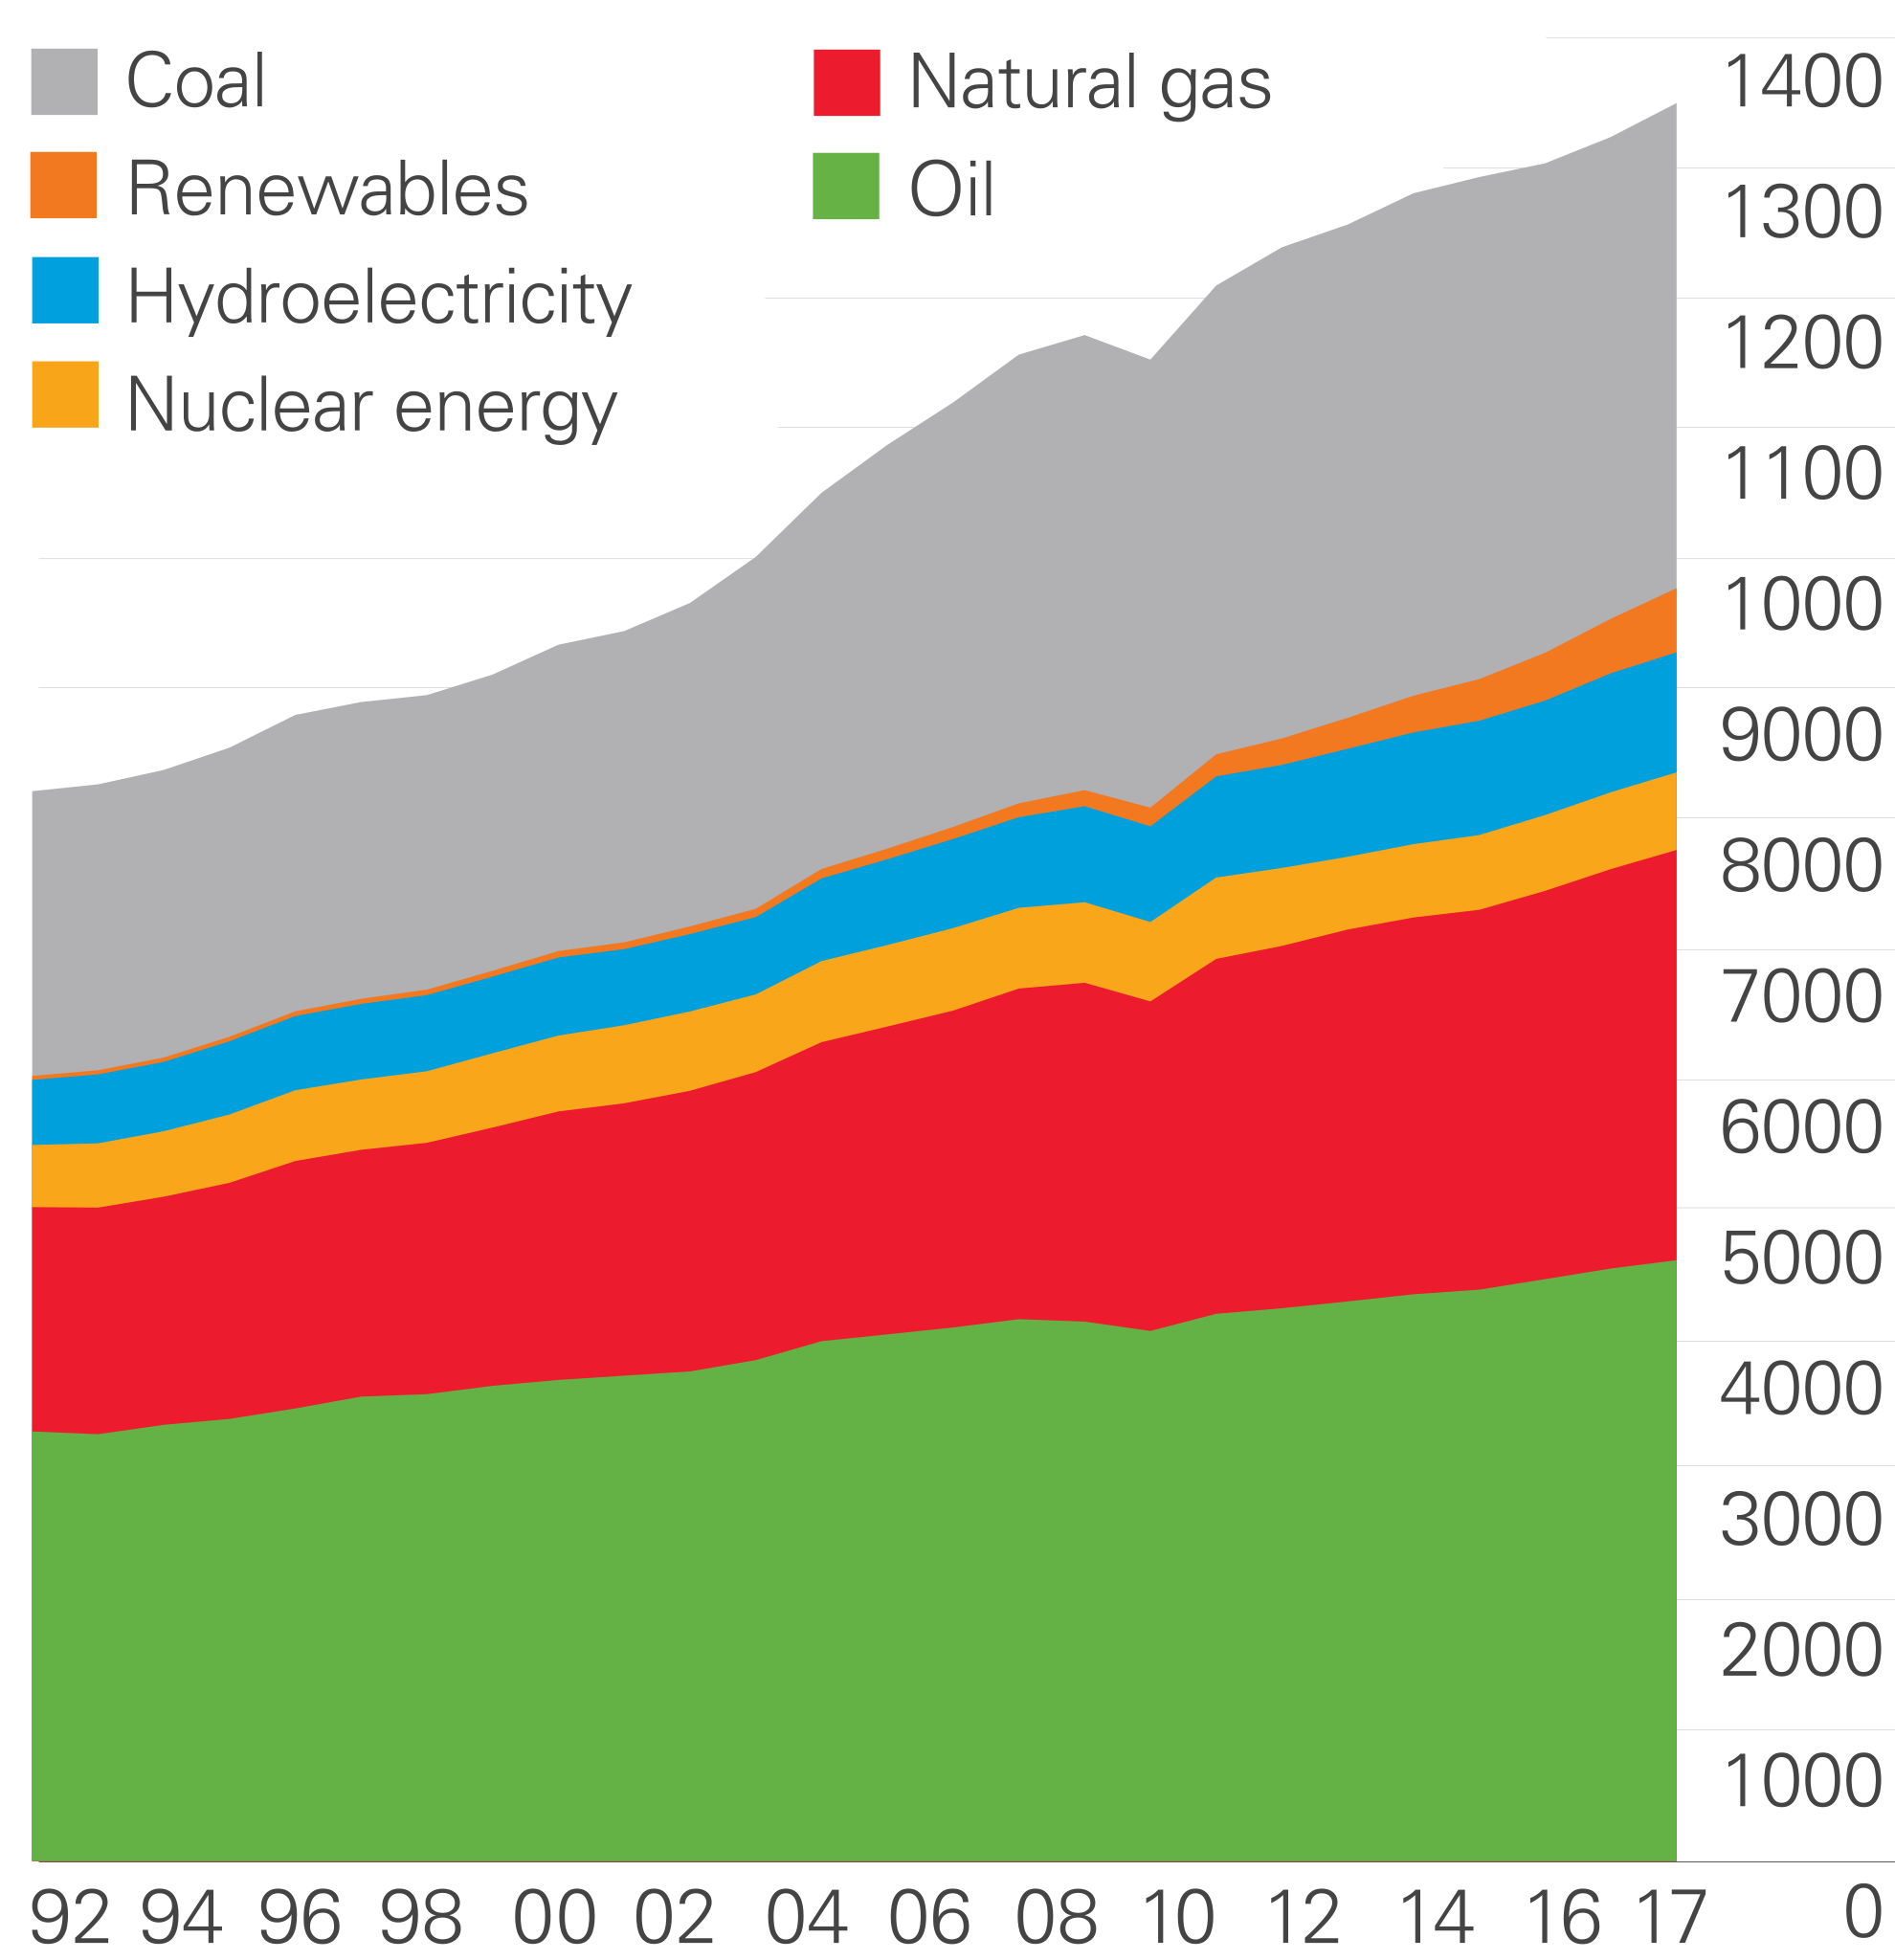
\includegraphics[scale=0.1]{globa_energy}
			\caption{Need to put a caption that will enusre the next level of text is in the next col}
		\end{figure}
		
		British Petroleum (BP) indicate coal, oil, and natural gas account for 85\% of goblal energy consumption \cite{BP:201806}. Energy from these fuels is generated from their combustion and is a major source of global greenhouse gas emissions which contribute to global warming \cite{Azapagic:2011}. In contrast, renewable sources of energy, which are comprised of wind, geothermal, solar, and biomass produce far fewer greehouse gas emissions, however, they only contribute a mere 3.5\% to global energy consumption. This is shown in a longitudinal breakdown, seen in Figure 1. The graph also shows that energy demand is increasing. If coal, oil, and natural gas remain core sources of generation then this will most likely result in greenhouse gas emissions rising, accelerating the rate of global warming. This is problematic given the well understood impacts global temperature increase has on the environment.\\
		
		The Intergovernmental Panel on Climate Change (IPCC) released a report in 2018 highlighting the link between greenhouse gas emissions and the increase in global temperatures citing human induced warming of 1$\si{\celsius}$ above pre-industrial levels in 2017, increasing at a minimum of 0.1$ \si{\celsius}$ per decade. The report forewarns of adverse environmental impact assuming maintained rates of CO2 emissions. These include an increase of 1.5$ \si{\celsius}$ above pre-industrial levels; increased frequency and intensity of heat waves; loss of biomass and a decrease in the number of species populations in climate sensitive areas; sea level rise; and food insecurity \cite{IPCC:2018}.\\ 
		
		Fortunately, the solar power industry is growing in Australia. As of September 2018, Australia had over 10131$\si{\mega\watt}$ of installed PV solar power. Approximately, 3366$\si{\mega\watt}$ were installed in the preceding 12 months \cite{APVI:2018}. In fact, the Australian renewable energy industry is on track to install more than 10$\si{\giga\watt}$ of new solar power during 2018 and 2019 - a rate which, if sustained, would see Australian generation reach 50\% renewables by 2025 \cite{Baldwin:2018}.\\
		
		Generation from large- and mid-sized solar arrays face the unique maintenance challenge of keeping the solar panels free from soiling. Soilng comes in the form of an accumutaion of dust, pollen, leaves, bird droppings or snail trails \cite{Maghami:2016}. An IBM research lab in 2018 demonstrated that Fully Convolutional Neural Networks can be used to help determine the soiling states of solar panels. Approximately 45000 images of solar panels in various states of soiling were collected. Trained models were successfully able to use object detection to locate the soiled regions of solar panels. Additionally, models could classify types of soiling, and provide an estimate of the power loss experienced by an individual panel \cite{Mehta:2018}.\\
		
		This paper proposes the use of a CNNs to classify images of solar panels as soiled or clean. A simple classification network like this could be used to set up an automatic visual inspection system, using drones equipped with RGB cameras, to determine soiling states for large solar arrays. This is of interest as it would allow scheduling of cleaning routines for maintenance cost optimisation. Cost savings would be realised reductions in labour required for manual visual inspections. Additionally, data could be used to determine optimal cleaning sequences for maximum power efficiency.\\
		
		\section{Background / Formulation}
		A Convolutional Neural Network (CNN) is a class of artificial neural network, which has an underlying architecture suited to learning shapes, edges, and colours in images. The main feature of a CNN is a convolving filter, which can be thought of as a small patch which slides over the image allowing model weights to be shared for different sections of the image. An example of this can be seen in Figure 2.\\
		\begin{figure}[h]
			\centering
			\includegraphics[scale=0.35]{CNN}
			\caption{An example of a convolutional layer - the small panel is convolved across the image producing the output (shown in blue).}
		\end{figure}
		
		CNNs are recognised as state-of-the-art methods for image classification, as seen in models such as GoogleNet \cite{Szegedy:2014}, ResNet \cite{He:2015}, and VGG \cite{Simonyan:2015}. Of course, recent CNNs, such as VGG, are very deep and contain a significant number of weights. This has two well understood effects:
		\begin{enumerate}
			\item High numbers of model weights requires more data to ensure that the model is adequately trained;
			\item Deep models dramatically increase the computation required for classification, making inference slower \cite{Cansiani:2017}.
		\end{enumerate}
		
		The second point is demonstrated pictorially, shown in Figures 3 and 4.
		
		\begin{figure}[h]
			\centering
			\includegraphics[scale=1]{tradeoff}
			\caption{A trade off exists between the number of operations, accuracy, and the number of parameters in a model.}
		\end{figure}
		
		\begin{figure}[h]
			\centering
			\includegraphics[scale=1]{tradeoff_2}
			\caption{Comparison of inference time versus batch size for different model architectures.}
		\end{figure}
		
		
		\clearpage
		\begin{figure*}[h]
			\centering
			\includegraphics[scale=1]{googlenet_arch}
			\caption{Googlenet architecture, with all the bells and whistles.}
		\end{figure*}
		\clearpage
		
		Given the lack of available image data for soiled solar panels, a model with too many parameters poses a risk of underfitting. This would yield poor classification results. Additionally, inference needs to be fast. A trained model deployed on a drone, used for soiling classification of a large solar panel array, will need to be able to process image data quickly. To help ensure performance requirements are met, some minimum benchmarks were perscribed for a secondary data set, not related to the solar panel classification problem. These include:
		\begin{enumerate}
			\item A hurdle rate of 75\% accuracy on model classification
			\item An inference speed of less than 10$\si{\milli\second}$ for a single image, given model deployment on [WHAT HARDWARE IS THIS]
		\end{enumerate}
		
		Googlenet was selected as the best model architecture Ready and available off the shelf that needed little to no development and amoung the state of the art model selections seemed to provide the best balance between model accuracy and inference time. It must be noted that this is most likely not the most optimal model - there is most likely some application specific model which would deliver superior performance and speed - this is similar to design choices when looking at embedded systems. For rapid system development the additional time and cost spent developing optimised systems means that the product may be redundant by the time that it is ready for release.
			
		\section{Data Acquisition}
		Image data was collected for threee distinct categories: clean solar panels, soiled solar panels, and images with no solar panels. Image data was aquired from Google images. Collection was automoated using a Python module called \verb|google_images_download|. Keywords used to search for each category can be seen in Table 1.
		\begin{table}[h]
			\centering
			\caption{Keywords used in Google Image searches.}
			\begin{tabular}{ll}
				\toprule
				\textbf{Classification Category} & \textbf{Keywords} \\
				\midrule
				Clean Solar Panels & \textit{Clean Solar Panels}\\
				 & \\
				Soiled Solar Panel & \textit{Dirty Solar Panel} \\
				 & \textit{Dusty Solar Panel} \\
				  & \\
				No Solar Panel & \textit{Roof} \\
				 & \textit{Rooftops} \\
				\bottomrule
			\end{tabular}
		\end{table}
		
		Each keyword search from the module returned 100 images, however, not all returned images were suitable and some were discarded during a manual review. This left 39 images for the Clean Solar Panel category; 102 images for the Soiled Solar Panel category; and  161 images for the No Solar Panel category. The final image sets were resized to 256$\times$256 - this introduced some distortion, due to unequal scaling, for those images that did not have square dimensions. Distortion could be avoided by image cropping, however, this would have added further complexity pre-processing.
		\begin{figure}[h]
			\centering
			\frame{\includegraphics[scale=0.5]{clean}}
			\caption{Example of an image of clean solar panels.}
		\end{figure}
		
		\begin{figure}[h]
			\centering
			\frame{\includegraphics[scale=0.5]{dirty}}
			\caption{An example of an image of soiled solar panels.}
		\end{figure}
		
		\begin{figure}[h]
			\centering
			\frame{\includegraphics[scale=0.5]{no_solar}}
			\caption{An example of an image of no solar panels.}
		\end{figure}
		
		Samples of images collected for the Clean Solar Panel, Soiled Solar Panel, and No Solar Panel can be seen in Figures 6, 7, and 8, respectively. The number of images for each class were doubled using a trick in which images are flipped from left to right and added back to the class. This resulted in a total of 604 images, broken downs as follows:
		
		\begin{itemize}
			\item \textbf{Clean solar panels:} 78
			\item \textbf{Dirty solar panels:} 204
			\item \textbf{No solar panels:} 322
		\end{itemize}
		
		The data was split into training and validation sets. Approximately 25\% of the images were held for the validation set.
		
		\section{Results}
		\subsection{Trial Data}
		To help analyse model performance independently of the solar panel data, the Googlenet model was trained on a trial data set consisting of approximately 10000 images. Images were split into training and validation sets with 9000 and 1000 images, respectiviely. The model was trained over 3 epochs using a batch size of 100. Reported accuracy was greater than 96\%, as shown in Figure 9. 
		\begin{figure}[h]
			\centering
			\includegraphics[scale=0.3]{trial_data_model_train}
			\caption{Googlenet trained using the trial dataset showed decreasing loss on training and validation sets. Accuracy was greater than 95\% on the third epoch.}
		\end{figure}
		
		Model performance was also evaluated against a set of unseen test data which resulted in an accuracy of 75.40\%. Further, the inference speed of the model was reported as approximately 5$\si{\milli\second}$.
		
		\subsection{Solar Panel Data}
		Model weights were re-initialised and the model re-trained using the solar panel image data set. Training was undertaken using 50 epochs with a batch size of 10. A higher number of epochs was used given that the data set was very small. Reported accuracy was approximately 80\%, as shown in Figure 10. 
		\begin{figure}[h]
			\centering
			\includegraphics[scale=0.3]{googlenet_train_img}
			\caption{Googlenet trained using the collected solar panel dataset showed decreasing loss on training and validation sets. Accuracy was approximately 80\% on epoch 50.}
		\end{figure}
		
		Trained model performance was evaluated against an unseen data set comprised of 15 images from each class. The model accuracy was reported as 62\%. A normalised confusion matrix can be seen in Figure XX.
		\begin{figure}[h]
			\centering
			\includegraphics[scale=0.37]{confusion_matrix}
			\caption{Confusion matrix showing reasonable classification performance for soiled and no solar panel categories, however, classification of clean solar panels was poor.}
		\end{figure}
			
		\section{Discussion}
		The Googlenet model trained on the trial dataset performed adequately, meeting the 75\% accuracy hurdle rate and an infernce speed almost twice as fast as the 10$\si{\milli\second}$ benchmark. The same cannot be said for the model performance on the solar dataset. Overall model accuracy is only 63\%. The confusion matrix highlights that the model had particular difficulty when attempting to classify a clean solar panel - it was in error 67\% of the time when classifying these image types. The most likely explanation for this poor performance is the lack of data for this class. Images of clean solar panels only make up approximately 12\% of the total images.\\
		
		The classification of soiled solar panels, and the classification of no solar panels performs notably better, as seen in the confusion matrix. It must be highlighted, however, that these positive results may be falsely inflated given the two classes represent a majority of the training data and there is a very clear distinction between images with solar panels, and images without solar panels. It is likely that introducing more clean solar panel images, whilst improving performance the clean solar panel class, will degrade performance when classifying soiled solar panels. Classification of no solar panel is likely to remain unchanged.\\
		
		As previously discussed, a solar panel soiling classificaiton experiment undertaken by IBM in 2018 which used object detection, performed significantly better than the results seen here. It must be noted, however, that the dataset for this experiment was much larger (approximately 45000 images) \cite{Mehta:2018}. It should also be noted that IBM's study obtained images from a fixed RGB camera pointed at a single solar panel system and the panel orientation remained unchanged throughout the experiment. In contrast, this experiment obtained images from Google of different sized solar systems viewed at varying angles. This suggests that the poor results may require a significant amount of data in order to train the model for reliable, robust performance.\\
		
		Finally, model hyperparameters such as the batch size, the number of epochs, and optimisation algorithms could be altered during the training phase, however, without a larger dataset the improvements to model performance are likely to be limited.
			
		\section{Conclusion / Future work}
		Googlenet provided a suitable framework for fast image classification, delivering a reasonable level of accuracy without compromising on inference speed. Model acccuracy of 75\% was achieved on a trial data set, while maintaining an inference time of 5$\si{\milli\second}$ for a single image. The application of a Googlenet architecture to the classification of 3 distinct soiling states for solar panels showed moderate performace for the no solar panel and the soiled solar panel test sets. Unfortunately, limited training dataset size meant the model did not generalise well on the final clean solar panel classification category.\\
		
		The development of a large dataset would likely prove the most fruitful approach to bolstering model performance for this application. Previous studies have used in excess of 45000 images for model training datasets resulting in reliable prediction of soiling state and an approximation of power loss for a single panel. One approach might be to partner with a large scale solar generation project and use aerial drones equipped with RGB cameras to capture more images of solar panels in known soiling states.
			
		\bibliography{my_bib}
		\bibliographystyle{ieeetr}
			
\end{document}